% Use the temporary template.
\documentclass[conference]{../aiaa-pretty}

% Author information
\author[Hastings, Dohnson, and Brooks]{ %
Edward N. Hastings\thanks{Graduate Research Assistant, Department of Aerospace Engineering, AIAA Student Member, \texttt{hastings@bysu.edu}},
David J. Dohnson\thanks{Graduate Research Assistant, Department of Aerospace Engineering, AIAA Student Member, \texttt{dohnson@bysu.edu}},
Gerlad R. Brooks\thanks{Professor, Department of Aerospace Engineering, AIAA Fellow, \texttt{brooks@bysu.edu}}\\
\textit{\small{Bowling Yellow State University, Springfield, MD 69743}}}

% Title
\title{An Improved Algorithm for Solving Equations of One Variable}

% Abstract
 \abstract{ %
  This paper demonstrates the use of a particular template.  In the mean time, it discusses algorithms to solve nonlinear equations of a single variable.  This is a subject that lends itself well to simple equations and the use of a few figures and tables.  This should be enough to demonstrate the main features of this package using a small number of pages.}

% Begin the document
\begin{document}
% Insert the title.
\maketitle 

\section{Introduction}
Many texts, for example \cite{chapra:2002:numerics}, have chapters on this subject.  We are motivated\footnote{Testing the footnote} to develop an accurate model for scramjet nozzles that runs in less than one second on a modern desktop computer.
\begin{equation}
x_{n+1} = x_n - \frac{f(x_n)}{f'(x_n)}
\end{equation}
Now we can see how the spacing works.

\section{Numerical Techniques}

\subsection{Convergence Criteria}
Figure \ref{fig:f:tol} gives a visualization for the uncertainty in both axes for several iterations of a bracketing scheme.  The yellow circles represent the iterative upper and lower bounds for the root location, and the sequentially darker orange boxes represent the current estimate of the region in which the root must exist.  Of course, we know that the root must lie on the $x$-axis, but the height of the box still gives a good representation of how good the current estimate is.

\begin{figure}
 \centering
 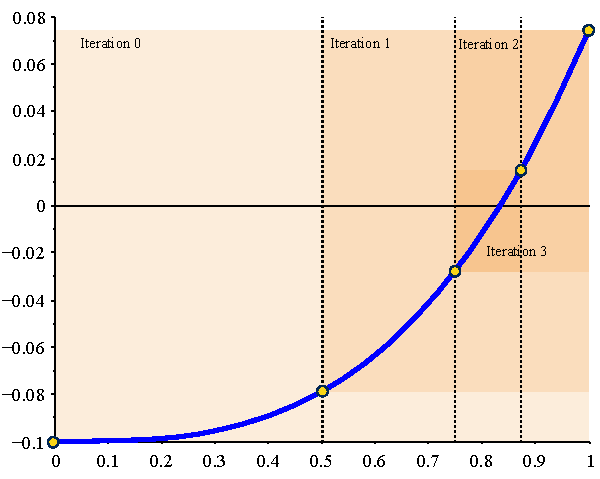
\includegraphics{./pics/f1_tol.pdf}
 \caption{ \label{fig:f:tol}
  Residuals in $x$- and $y$-directions}
\end{figure}



\section{Results}

\section{Conclusions}                            \label{sec:conclusion}
A reduced-order two-dimensional model was developed that can analyze shock waves, expansion fans, and finite-rate chemistry.  The model was found to be particularly accurate in determining the boundary of the exhaust plume, which is essential to thrust calculations.  Recombination can also be modeled as long as the flow is well-mixed before reaching the nozzle.  However, the importance of recombination to thrust calculations was debatable, even for a set of conditions specifically selected to emphasize the importance of recombination.

The model does not have the capability to analyze boundary layers, which were found to play an important role.  The boundary layer had a noticeable effect on all quantities except for pressure.  These results make a strong case that a boundary layer model must be added to the reduced-order model.

\begin{figure}[!h]
 \begin{center}
  Whatever
 \end{center}
 \caption{Test figure}
\end{figure}

\section*{Acknowledgements}
This document was prepared by Derek Dalle with help from Sara Spangelo.

% References
\bibliographystyle{aiaa}
\bibliography{./bib/aiaa-sample}


\end{document}
